\chapter{CoNtRoL Simulations Web Application}
\label{conclusions}

//TODO: s-a cam schimbat totu lmao lol

\par
\textit{ Here we will present the open-source Web application developed for easing work involving chemical reaction networks, hopefully for students and researchers one day. It can be used for obtaining numerical analysis of chemical reaction networks, as well as plotting species against time, one another and so on. We'll present the technologies used throughout the project, how to run it locally and a couple of usage examples involving what we've presented in the previous chapters. }

\subsection{Overview of the technologies}
The website is a back-end application built in \textbf{Python}, a programming language known for its use in basically every single science, including natural sciences so it's a no-brainer when in comes to plotting.

The web server is built using \textbf{Flask}, a lightweight web app framework and the webpages served are server-side rendered by Flask's template engine depedency - \textbf{Jinja}.
\\
The crux of the functionality is aided by the Python library \textbf{Tellurium}; which is, as their docs say; "A Python Environment for Reproducible Dynamical Modeling of Biological Networks". It uses a subset of the Systems Biology Markup Language ( \textbf{SBML}) called \textbf{Antimony} which can be used in this app to create a Chemical Reaction Network, as well as the friendlier selects form. So the bits doing the magic are the calls to \verb|road_runner.loada()| which are used to \textbf{\textit{load}}    \textbf{a}ntimony code into the model.
the \verb|road_runner..simulate()| function is then used for running and obtaining sumulation data, followed by \verb|road_runner.plot()|, which in turn calls a \verb|matplotlib| headless backend for writing the plotted results to a file.

\subsection{Running it}
As explained in the \verb|README| of \href{https://github.com/viktorashi/Open-CoNtRol}{the project}, running locally is done automatically by the \verb|run_script.sh|, which figures out your machine's local IP, sets the required environment variables and runs \\

\verb|flask --debug run --host="$ip"|. Output regarding traffic to the server as well as internal workings of the app will now be redirected to \verb|stdout| of the terminal. \\\\\\\\\\
All the user has to do beforehand is:

\tikz\draw[black,fill=black] (0,0) circle (.5ex); clone the project

\begin{lstlisting}[language=bash]
    git clone https://github.com/viktorashi/Open-CoNtRol.git
\end{lstlisting}

\tikz\draw[black,fill=black] (0,0) circle (.5ex); \textbf{c}hange \textbf{d}irectory into it.

\begin{lstlisting}[language=bash]
    cd Open-CoNtRol
\end{lstlisting}

\tikz\draw[black,fill=black] (0,0) circle (.5ex); install the requirements

\begin{lstlisting}[language=bash]
    pip install -r requirements.txt
\end{lstlisting}

\tikz\draw[black,fill=black] (0,0) circle (.5ex);
give the \verb|run_script.sh| execute permissions

\begin{lstlisting}[language=bash]
    chmod +x ./run_script.sh
\end{lstlisting}

\tikz\draw[black,fill=black] (0,0) circle (.5ex);
and finally run it

\begin{lstlisting}[language=bash]
    ./run_script.sh
\end{lstlisting}

Among the wall of output will also be the line showing the address your server is located at, for example:
\verb|* Running on http://192.168.0.94:5000|, address at which you'll be greeted with this screen

\[
	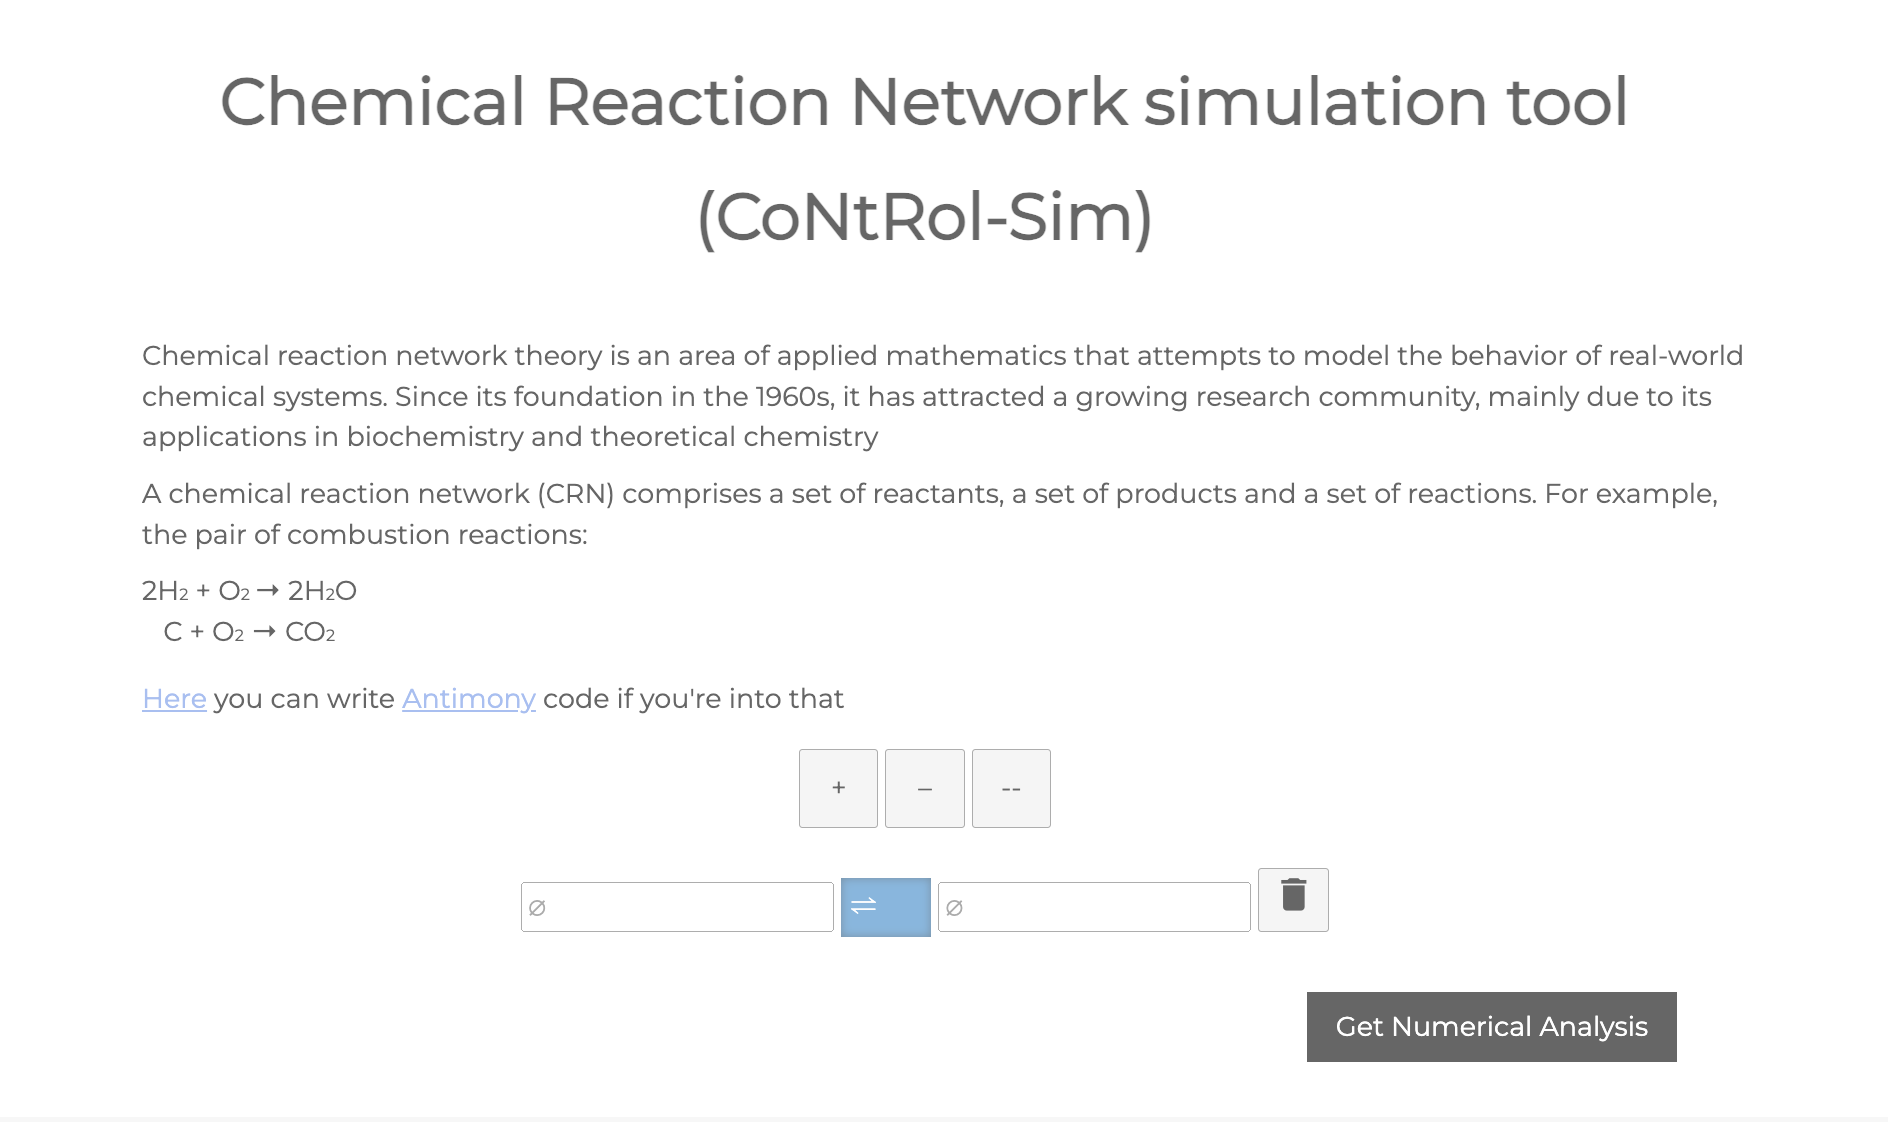
\includegraphics[width=13cm]{app_photos/control_home_screen.png}\\
\]

You can either use this as a starting point or the page located at the \verb|/antimony| path:

\[
	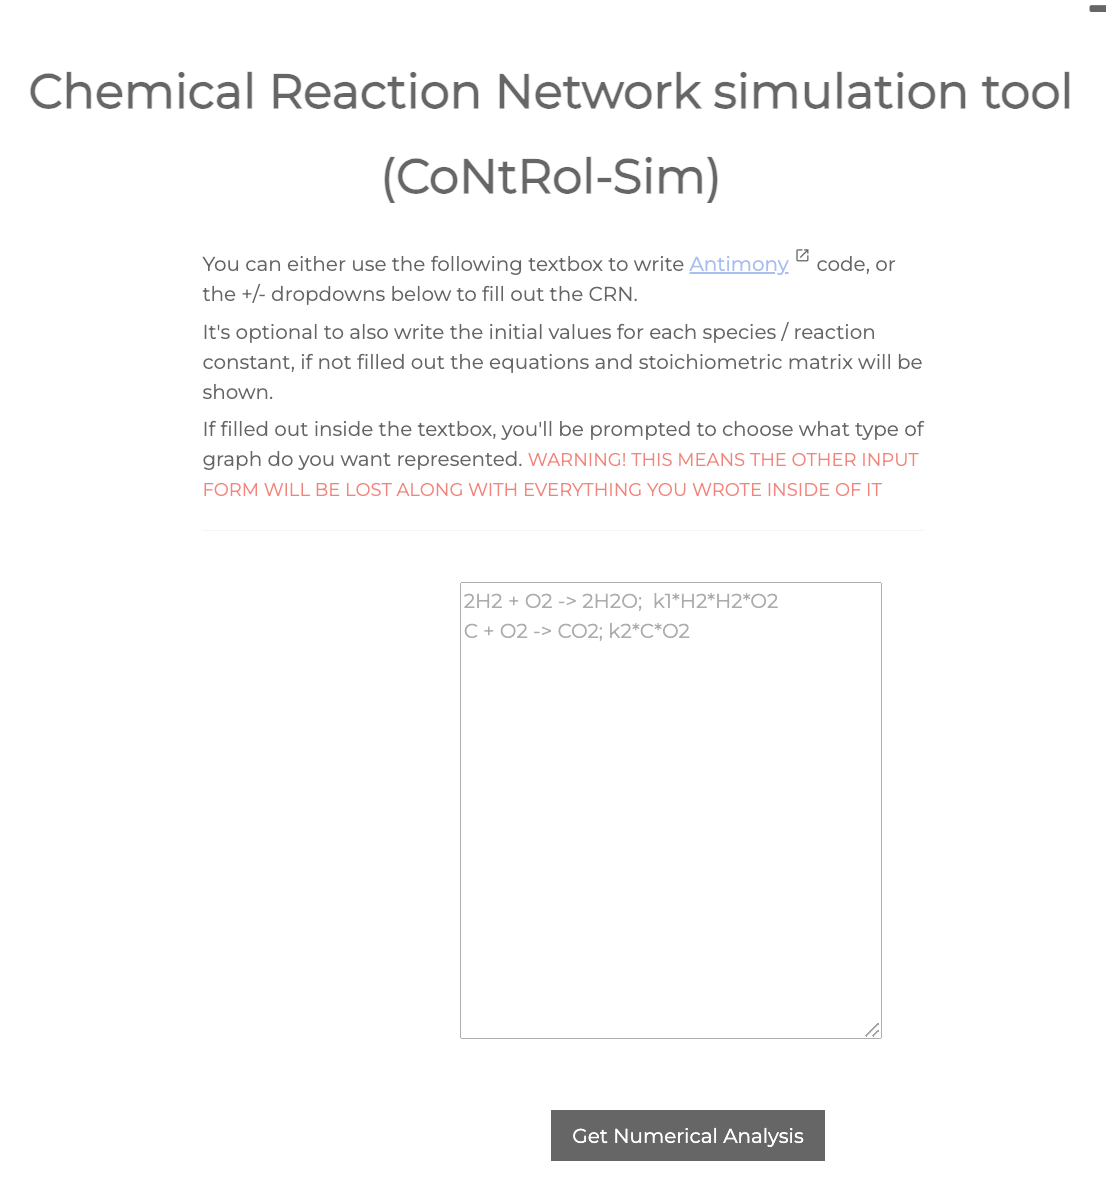
\includegraphics[width=13cm]{app_photos/control_antimony_home.png}\\
\]
Both of these redirect to \verb|/numerical_analysis| analysing the system \ldots well, numerically.
As an example, this Antimony code:

\begin{lstlisting}
S0 -> KS1; k1*S0
KS1 -> S2; k2*KS1
S2 + F -> FS2; k3*S2*F
FS2 -> F; k4*FS2
F -> S0 + F; k5*F
\end{lstlisting}

and its longer to write alternative:

\[
	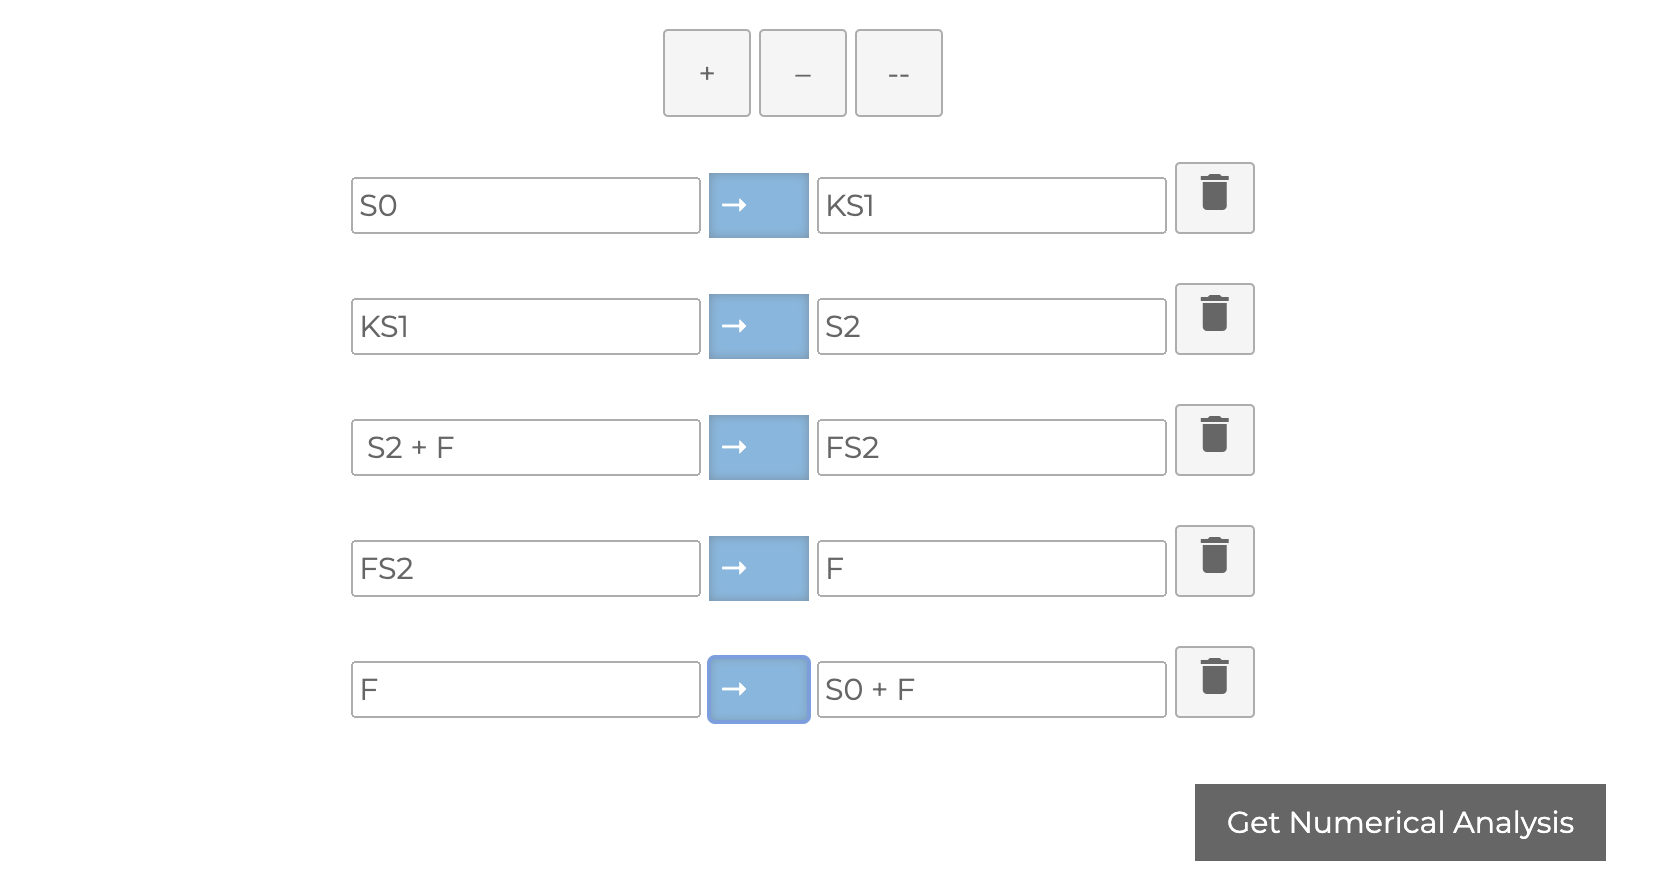
\includegraphics[width=13cm]{app_photos/creca-prima-data-cand-am-scris-asta.png}\\
\]

both yield the same numerical analysis results:

\[
	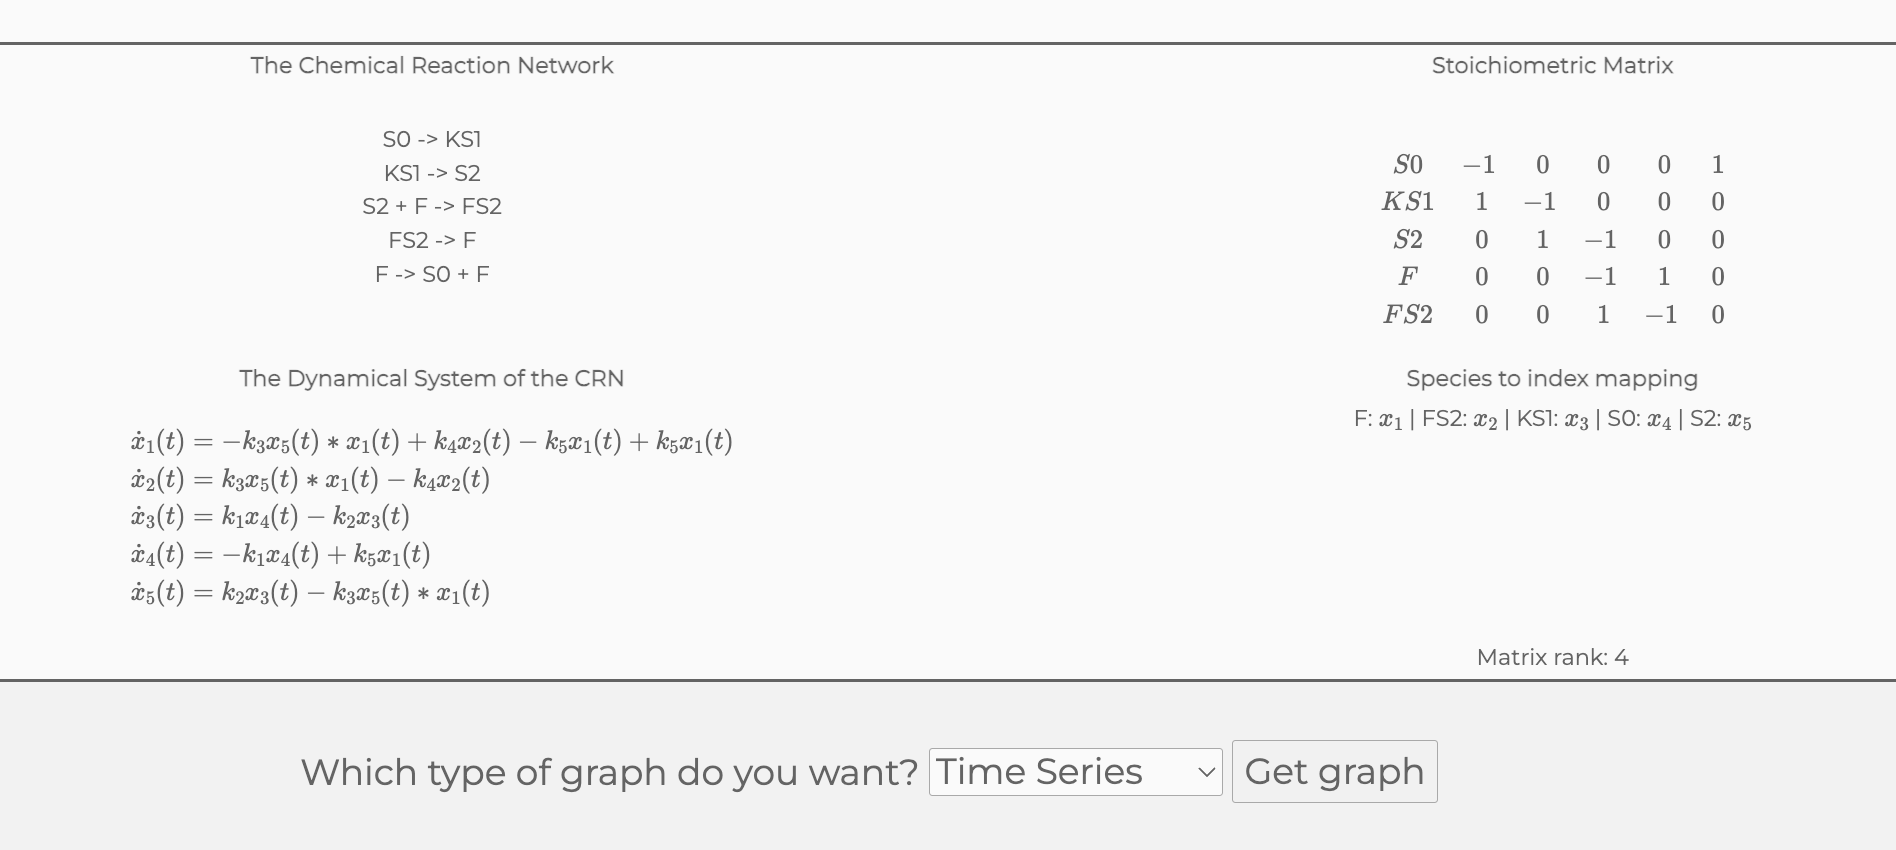
\includegraphics[width=13cm]{app_photos/numerical_analysis.png}\\
\]

from here, one can choose from a selection of graphs they can represent given this system, the default one being the time series representation:

\[
	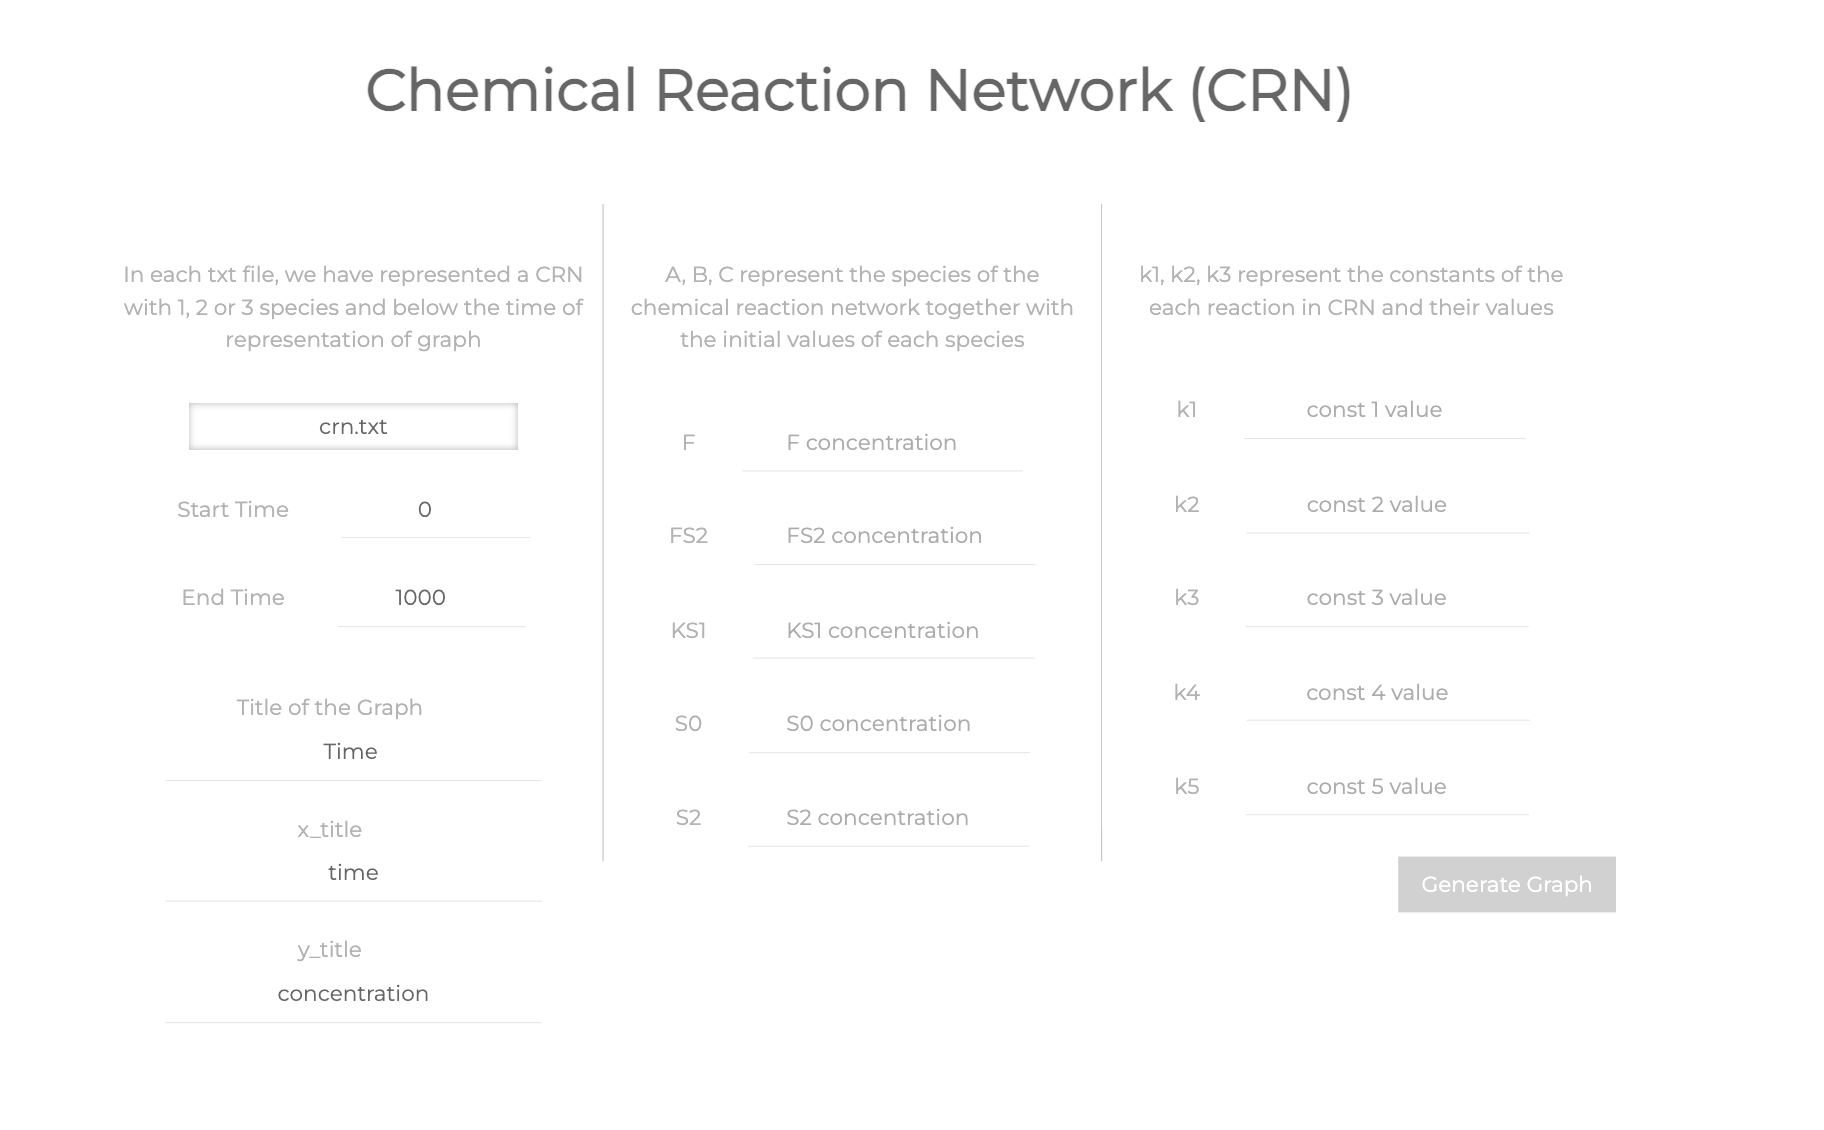
\includegraphics[width=13cm]{app_photos/tsr-input.png}\\
\]

from which we fill out the initial values of the concentrations for each species as, well as the reaction rates. So given, for example the values:

\begin{lstlisting}
    F = 0.874108
    FS2 = 7.620157734
    KS1 = 7.620157734
    S0 = 7.270157734
    S2 = 0.6000000000

    k1 = 0.1329759342
    k2 = 0.1329759342
    k3 = 2
    k4 = 0.1329759342
    k5 = 1
\end{lstlisting}

outcomes the graph:

\[
	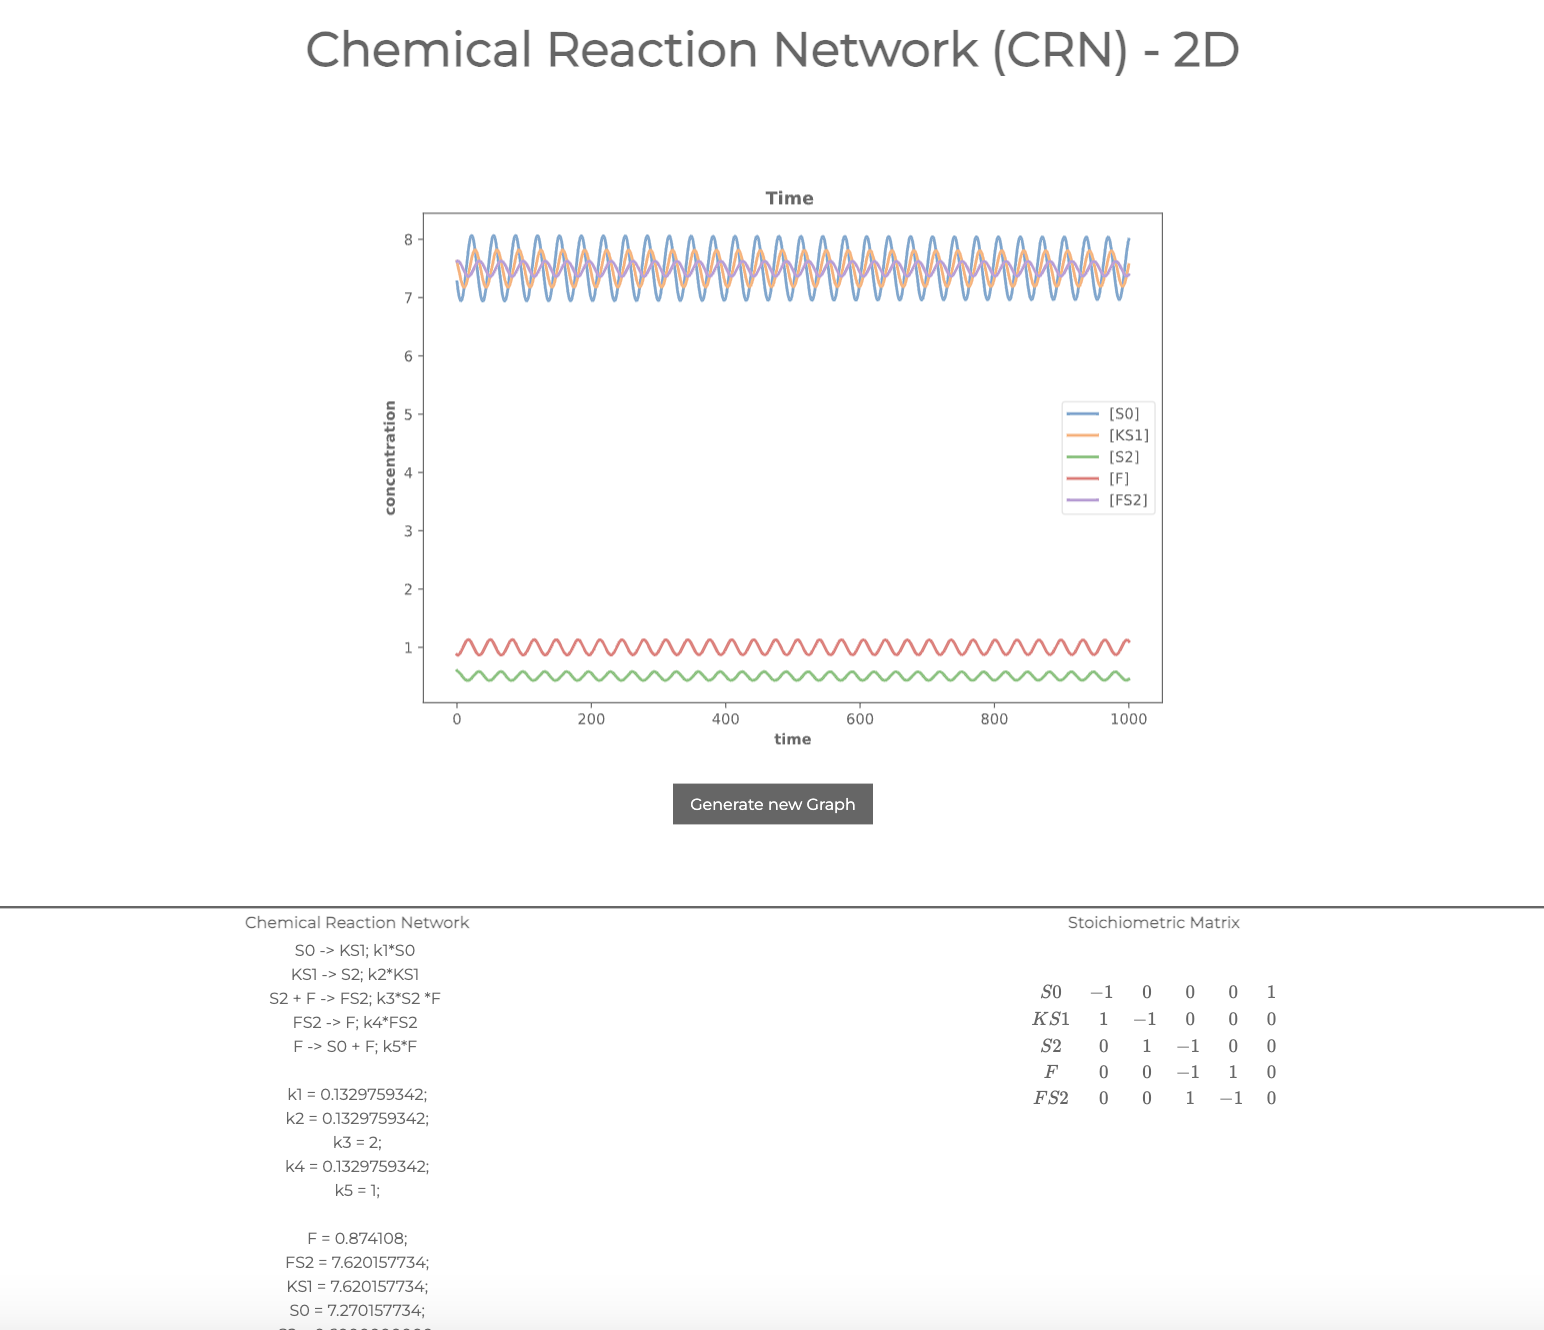
\includegraphics[width=13cm]{app_photos/a-graph-indeed.png}\\
\].

\subsection{The bottom line}

So this is how the workflow of the app typically goes. \\
$
\begin{WithArrows} & \textit{write out your system} \rightarrow \textit{get numerical analysis} \rightarrow \textit{choose your desired graph} \Arrow{\textit{fill out data values}}  \\
	& \hfill \textbf{Voilà}
\end{WithArrows}
$
